\section{Økonomisk analyse}

Denne seksjonen tallfester kostnadsbildet, inntektsgrunnlaget og
break-even-kravene som kontrollrammeverket i seksjon~7 peker mot.
Tallene bygger på offentlige referansekilder der de finnes, og på
sammenlignbare operasjoner hos Aviant i Norge, Zipline i USA og
markedsdata for tilsvarende VTOL-droner der tallene ikke er offentlige.
Antagelsene dokumenteres fortløpende, og resultatene presenteres som
grove størrelsesordener som må justeres når faktiske driftstall
foreligger.

\subsection{Investering og driftskostnader i piloten}

Pilotfasen på Nesodden krever både en initiell investering (CAPEX) og
en løpende drift (OPEX). Størrelsen bestemmes av flåtestørrelse, base,
godkjenninger og en kjerne av operasjonelt personell.

\paragraph{CAPEX.}
En pilotflåte på fem VTOL-droner i klassen under 5~kg nyttelast koster
anslagsvis 85~000~USD per drone \parencite{hinaray2025}, altså rundt
4,5~MNOK for hele flåten ved en kurs på 10,5~NOK/USD. Oppsett av
ladestasjon, lagringshub og software-integrasjon ved Alti Vinterbro
anslås til rundt 1,5~MNOK basert på industribenchmark for
distribusjonssentre i samme kategori \parencite{konapur2025, freightamigo2025}.
Regulatorisk godkjenning i spesifikk kategori innebærer et årsgebyr på
20~000~kr til Luftfartstilsynet pluss saksbehandlingsgebyr etter regning
\parencite{luftfartstilsynet2026, uasnorway2025_gebyr}. Hovedkostnaden
ligger likevel i ekstern rådgivning og teknisk dokumentasjon for
SORA-vurdering, BVLOS-søknad og sikkerhetsanalyse, som for
sammenlignbare oppstartsprosjekter i Europa antas å ligge i området
0,5--1,0~MNOK. Tallet er et estimat, og faktisk kostnad bestemmes av
omfanget av operasjonen og graden av intern fagkompetanse hos Zipline.
Sammen med en reserve for uforutsette kostnader lander samlet
pilot-CAPEX på 6--8,5~MNOK.

\paragraph{Fast OPEX.}
Piloten krever fem heltidsstillinger, altså pilotprosjektleder,
operasjonsansvarlig, markedsansvarlig, partneransvarlig og tekniker.
Gjennomsnittlig lønn for tilsvarende stillinger i teknologibedrifter i
Norge ligger rundt 800~000~kr per år, og inkludert arbeidsgiveravgift,
pensjon og feriepenger blir samlet arbeidskraftkostnad anslagsvis
1,0~MNOK per årsverk \parencite{ssb2024}. Fem stillinger gir dermed rundt 420~k per måned i lønn. Base-leie for
et hub- og kontorareal på 150--200~m² ved Vinterbro anslås til
25--40~k per måned, basert på leiepriser for næringslokaler i randsonen
av Oslo-regionen på 1\,800--2\,300~kr per kvadratmeter per år
\parencite{spacefinder2025}. Ansvarsforsikring er lovpålagt for
kommersiell droneoperasjon i Norge \parencite{coverdrone2025,
luftfartstilsynet2026}, men prises individuelt basert på flåtestørrelse
og operasjonsprofil. Den anslås til 15--30~k per måned for en flåte på
fem droner i BVLOS-drift. Markedsbudsjett i piloten er satt til 150~k
per måned som en strategisk beslutning framfor et kildebelagt tall, og
reflekterer typiske B2C-lanseringsandeler hos teknologistartups.
Samlet fast OPEX lander dermed på 610--740~k per måned.

\paragraph{Variabel OPEX.}
Per leveranse dominerer energi og vedlikehold. Platform~2 bruker
anslagsvis 97~\% mindre energi enn bilbasert levering
\parencite{electrek2023}, noe som tilsvarer 1--2~kWh per
tur-retur-levering. Ved norsk bedriftsstrøm på rundt 100~øre/kWh
\parencite{ssb2025_elektrisitet, fortum2025_strom} blir
energikostnaden 1--2~kr. Vedlikehold er den viktigste kilden til
usikkerhet. Zipline anslår kostnaden per leveranse til 2--4~USD ved
moden drift \parencite{dronexl2026}, men piloten opererer på lavt
volum der slitasje allokeres over få leveranser. Et realistisk
pilot-anslag er 30--45~kr per leveranse, med forventning om at
kostnaden faller mot 20~kr i fase~3 og fase~4 etter hvert som volumet
skaleres.

\begin{table}[H]
\centering
\caption{Kostnadsbilde for pilotfasen}
\label{tab:pilotkostnader}
\renewcommand{\arraystretch}{1.2}
\begin{tabularx}{\textwidth}{@{} l X r @{}}
\toprule
\rowcolor{tableheader}
\color{white}\textbf{Post} & \color{white}\textbf{Beskrivelse} &
\color{white}\textbf{Beløp} \\
\midrule
CAPEX flåte & 5 VTOL-droner à 85~000~USD & 4,5~MNOK \\
CAPEX hub & Launchpad, lade, lager, software & 1,5~MNOK \\
CAPEX regulatorisk & SORA- og BVLOS-sertifisering & 0,75~MNOK \\
CAPEX reserve & Uforutsette kostnader & 0,5~MNOK \\
\midrule
Fast OPEX/mnd & Lønn, leie, forsikring, marked & 610--740~k \\
Variabel OPEX/lev. & Energi og vedlikehold (pilot-skala) & 30--45~kr \\
\bottomrule
\end{tabularx}
\end{table}

\subsection{Inntektsmodell og betalingsvilje}

Inntektene kommer fra to hovedkilder. Den første er leveringsgebyret
kunden betaler per ordre. Den andre er partnerprovisjonen Zipline tar
fra innholdspartnere som Coop Obs og Jordbærpikene for å formidle
bestillingen. Serviceavgift er en mulig tredje inntektskilde, men
holdes utenfor piloten for å gjøre prissignalet mot kunden enkelt.

\paragraph{Pris-benchmark.}
Foodora har i Oslo et gjennomsnittlig leveringsgebyr på 59~kr, med
eksempler ned i 49~kr for sentrale bydeler
\parencite{allrestaurantmenus2026}. Wolt tilbyr gratis levering ved
bestilling over 165--375~kr eller via Wolt+ til 99~kr per måned
\parencite{wolt2025_levering}. I USA leverer Zipline for 0,99~USD i leveringsgebyr pluss 20~\%
serviceavgift oppad begrenset til 6~USD \parencite{stevens2025}, den
samme prismodellen som ligger til grunn for posisjoneringen i
seksjon~6. Ved en valutakurs på 10,5~NOK/USD utgjør leveringsgebyret
alene rundt 10~kr. Serviceavgiften på 20~\% av bestillingsverdien gir
30--40~kr for typiske bestillinger på 150--200~kr, altså et samlet
tillegg til kunden på 40--50~kr utover bestillingsverdien. Posisjoneringen i seksjon~6
peker på at Zipline skal være rimeligere enn Foodora og Wolt, og en
leveringspris på 29~kr gir et klart differensieringssignal mot
Foodoras typiske 49--59~kr.

\paragraph{Betalingsvilje.}
Fokusgruppen rapporterer høy prissensitivitet, og deltakerne stilte
eksplisitt som betingelse at Zipline må være lik eller lavere i pris
enn alternativet (vedlegg~B). Spørreundersøkelsen (vedlegg~A) viser at
primærsegmentet K4 er svært prissensitivt, men samtidig har høyest
drone-vilje (62~\%), og at både K1 og K3 rangerer pålitelighet og lav
pris som sine viktigste kriterier. Både kvantitativ og kvalitativ data
støtter dermed en pris tydelig under Foodora-nivået. Partnerprovisjonen
settes til 25~\% av bestillingsverdien, noe som ligger i nedre sjikt
av bransjen. Foodora tar typisk 30--35~\%
\parencite{aftenbladet2024_foodora}, og Wolt 20--30~\%
\parencite{menuviel2025_wolt}. En lavere sats gjør Zipline mer
attraktiv for partnerne i oppstartsfasen. Snittbestilling antas å
ligge rundt 250~kr basert på typisk ordreverdi i matlevering og
dagligvare i Norge, uten at et offentlig referansetall foreligger.
Samlet inntekt per leveranse blir dermed 29~kr pluss 25~\% av 250~kr,
altså rundt 91~kr.

\subsection{Fase 1 -- Bærum og Asker}

Fase 1 er Ziplines første kommersielle ekspansjon utenfor Nesodden og
dekker Bærum (132\,358 innbyggere per Q4 2024) og Asker (101\,509
innbyggere per Q4 2025) \parencite{ssb_kommunefakta_baerum,
ssb_kommunefakta_asker}. Med en gjennomsnittlig husholdningsstørrelse
på 2,29 personer \parencite{ssb_kommunefakta_asker} tilsvarer dette om
lag 103\,000 husholdninger i kombinert markedsgrunnlag. Statista anslår
samlet penetrasjonsrate for dagligvarelevering i Norge til 39,8~\% i
2024 \parencite{statista2024_grocery_norway}, fordelt på etablerte
aktører som Foodora og Wolt.

\paragraph{Volumantagelser.}
Ziplines mål i fase 1 er å ta en liten, men meningsfull andel av dette
markedet. Ved utgangen av fase 1 antas 3~\% av husholdningene å være
aktive brukere (om lag 3\,100 kunder), hver med 1,5 bestillinger per
måned i snitt. Dette gir et måltvolum på rundt 4\,000 leveranser per
måned. Antallet bygges opp gradvis fra pilot-nivået på 500--700
leveranser ved oppstart til 4\,000 ved slutten av fase 1, i tråd med
Rogers' adopsjonskurve for nye tjenester \parencite{rogers2003}.

\paragraph{Inkremental CAPEX.}
Fase 1 krever utvidet flåte og en ny driftsbase nærmere Bærum.
Flåtebehovet beregnes fra et effektivt kapasitetsanslag på rundt 8
leveranser per drone per operativ dag (12 nominelle leveranser minus
30~\% fratrekk for vær og vedlikehold) eller om lag 240 per måned.
For å håndtere 4\,000 leveranser per måned med reservekapasitet
trenger Zipline 17--20 droner totalt, altså 12--15 nye ut over
pilot-flåten. Ved 85\,000~USD per drone gir dette en ekstra
drone-investering på 10,7--13,4~MNOK \parencite{hinaray2025}. En ny hub
i Bærum med launchpad, lading og lager anslås til 2,5~MNOK, og utvidet
regulatorisk godkjenning til 0,5~MNOK. Samlet inkremental CAPEX lander
dermed på 13--16~MNOK.

\paragraph{Fast OPEX.}
Organisasjonen utvides med tre til fem stillinger utover pilotens fem,
hovedsakelig operatører og partneransvarlige, noe som gir en
lønnskostnad på rundt 900~k per måned. Base-leie for Bærum-hub
(tilsvarende 150~m² på Akershus-nivå) anslås til 25--35~k per måned
\parencite{spacefinder2025}, forsikring for den utvidede flåten til
40~k per måned, og markedsbudsjett til 300~k per måned for å bygge
merkevare og konvertere tidligbrukere. Samlet fast OPEX i fase 1
lander på rundt 1,2~MNOK per måned.

\subsection{Fase 2 -- Vestre Aker og Holmenkollen}

Fase 2 utvider dekningen til Bydel Vestre Aker, som hadde 51\,487
innbyggere i 2023 \parencite{oslo_bydelsfakta_vestreaker}. Med en
gjennomsnittlig husholdningsstørrelse på rundt 2,1 personer i Oslos
vestlige bydeler tilsvarer dette om lag 24\,500 husholdninger.
Bydelen omfatter blant annet Holmenkollen, Slemdal og Vinderen, der
målrettingen i seksjon~6 peker på en eldre og mer adopsjonskrevende
kundegruppe. SSB viser at aldersgruppen over 67 år er tregere med å ta
i bruk nye digitale tjenester \parencite{ssb2023}, og
ambassadørprogrammet i fase 2 er utformet for å håndtere nettopp
dette.

\paragraph{Volumantagelser.}
Ved utgangen av fase 2 antas 2~\% av husholdningene i Vestre Aker å
være aktive (om lag 490 kunder), som med 1,5 bestillinger per måned
gir 735 ordre per måned fra det nye området. I tillegg fortsetter
veksten i Bærum og Asker. Samlet volum bygges fra 4\,000 ved slutten
av fase 1 til om lag 7\,800 leveranser per måned ved slutten av fase
2. Den lavere adopsjonsraten i Vestre Aker reflekterer både målgruppens
høyere terskel og at ambassadørprogrammet skalerer dårligere enn
digital kampanje per påløpt krone.

\paragraph{Inkremental CAPEX.}
For å betjene et samlet volum på 7\,800 leveranser per måned trengs
32--35 droner, altså 12--15 nye ut over fase 1-flåten. Dette gir en
ekstra drone-investering på 10,7--13,4~MNOK \parencite{hinaray2025}.
Pilot- og Bærum-hubbene dekker i utgangspunktet geografien, men
driften kan trenge justeringer i launchpad-kapasitet, anslått til
0,5~MNOK. Samlet inkremental CAPEX i fase 2 er rundt 11~MNOK.

\paragraph{Fast OPEX.}
Organisasjonen utvides videre med tre til fire stillinger, blant
annet en dedikert relasjonsansvarlig for ambassadørprogrammet. Dette
gir en lønnskostnad på rundt 1,2~MNOK per måned totalt. Base- og
forsikringskostnader øker moderat med flåten til rundt 90~k per måned
kombinert. Markedsbudsjettet holdes på 450--500~k per måned,
fordelt mellom videreføring av fase 1-kampanjen i Bærum og
ambassadør- og relasjonsarbeidet i Vestre Aker. Samlet fast OPEX i
fase 2 lander på rundt 1,8~MNOK per måned.

\subsection{Akkumulert kontantstrøm over 24 måneder}

Akkumulert kontantstrøm bygges opp fra pilotens startposisjon og
følger volumets S-formede opptrapping gjennom fase 1--4. Hver måned
beregnes som \((p - v) \cdot Q_t - F_t\), der \(Q_t\) er månedens
volum, \(v\) er variabel kostnad per leveranse, \(p\) er inntekt per
leveranse, og \(F_t\) er fast OPEX per måned. Ved overgangen mellom
faser legges inkremental CAPEX til som et engangsbeløp. Startpunktet
ved måned 0 er pilotens akkumulerte underskudd på rundt 15~MNOK
(7,5~MNOK CAPEX og 7,8~MNOK operativt tap over 12 måneder).

Parametrene er oppsummert i tabell~\ref{tab:faseparams}, og resulterer
i kontantstrømkurven i figur~\ref{fig:kontantstrom}.

\begin{table}[H]
\centering
\caption{Parameterantagelser per fase i kontantstrømanalysen}
\label{tab:faseparams}
\renewcommand{\arraystretch}{1.2}
\begin{tabularx}{\textwidth}{@{} l X r r r r @{}}
\toprule
\rowcolor{tableheader}
\color{white}\textbf{Fase} & \color{white}\textbf{Område} &
\color{white}\textbf{Vol. slutt} & \color{white}\textbf{Var.} &
\color{white}\textbf{Fast} & \color{white}\textbf{CAPEX} \\
\midrule
Pilot  & Nesodden          &    700 & 40 & 0,7 & 7,5  \\
Fase 1 & Bærum og Asker    &  4\,000 & 30 & 1,2 & 14,0 \\
Fase 2 & Vestre Aker       &  7\,800 & 25 & 1,8 & 11,0 \\
Fase 3 & Konsolidering     & 14\,000 & 20 & 2,5 & 5,0  \\
Fase 4 & Nasjonal (Trondheim) & 40\,000 & 18 & 4,0 & 15,0 \\
\bottomrule
\end{tabularx}
\end{table}

Volumkolonnen viser volum (leveranser per måned) ved slutten av fasen,
variabel kostnad er kr per leveranse, fast OPEX er MNOK per måned, og
CAPEX er inkremental investering i MNOK ved fasens start.

\begin{figure}[H]
\centering
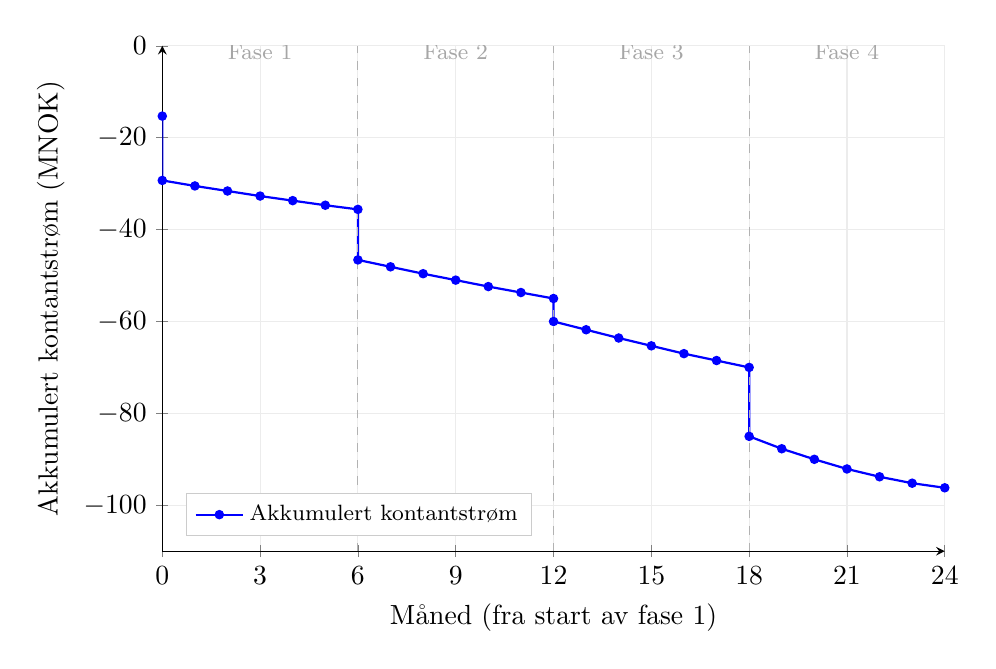
\begin{tikzpicture}
\begin{axis}[
    width=0.95\textwidth,
    height=8cm,
    xlabel={Måned (fra start av fase 1)},
    ylabel={Akkumulert kontantstrøm (MNOK)},
    xmin=0, xmax=24,
    ymin=-110, ymax=0,
    legend pos=south west,
    legend style={font=\footnotesize, fill=white, draw=gray!40},
    grid=major,
    grid style={gray!15},
    axis lines=left,
    xtick={0, 3, 6, 9, 12, 15, 18, 21, 24},
    ytick={0, -20, -40, -60, -80, -100},
]
\addplot[thick, blue, mark=*, mark size=1.3pt] coordinates {
    (0,  -15.3)
    (0,  -29.3)
    (1,  -30.5)
    (2,  -31.6)
    (3,  -32.7)
    (4,  -33.7)
    (5,  -34.7)
    (6,  -35.6)
    (6,  -46.6)
    (7,  -48.1)
    (8,  -49.6)
    (9,  -51.0)
    (10, -52.4)
    (11, -53.7)
    (12, -55.0)
    (12, -60.0)
    (13, -61.8)
    (14, -63.6)
    (15, -65.3)
    (16, -67.0)
    (17, -68.5)
    (18, -70.0)
    (18, -85.0)
    (19, -87.7)
    (20, -90.0)
    (21, -92.1)
    (22, -93.8)
    (23, -95.2)
    (24, -96.2)
};
\addlegendentry{Akkumulert kontantstrøm}

\draw[dashed, gray!60] (axis cs:6, -110) -- (axis cs:6, 0);
\draw[dashed, gray!60] (axis cs:12, -110) -- (axis cs:12, 0);
\draw[dashed, gray!60] (axis cs:18, -110) -- (axis cs:18, 0);
\node[anchor=south, font=\footnotesize, gray!70] at (axis cs:3, -5)
    {Fase 1};
\node[anchor=south, font=\footnotesize, gray!70] at (axis cs:9, -5)
    {Fase 2};
\node[anchor=south, font=\footnotesize, gray!70] at (axis cs:15, -5)
    {Fase 3};
\node[anchor=south, font=\footnotesize, gray!70] at (axis cs:21, -5)
    {Fase 4};
\end{axis}
\end{tikzpicture}
\caption{Akkumulert kontantstrøm fra start av fase 1 til slutt av fase
4. Vertikale hopp ved måned 0, 6, 12 og 18 reflekterer inkremental
CAPEX ved overgangen mellom fasene. Ved måned 24 ligger akkumulert
kontantstrøm på om lag --96~MNOK, og månedlig operativt underskudd
avtar etter hvert som volumet skaleres.}
\label{fig:kontantstrom}
\end{figure}

Kurven viser at akkumulert kontantstrøm er negativ gjennom hele den
toårige ekspansjonsperioden. Ved måned 24 har Zipline investert om
lag 96~MNOK totalt (inkludert pilot), fordelt på 52~MNOK kumulativ
CAPEX og 44~MNOK kumulativt operativt underskudd. Månedlig operativt
underskudd topper seg i midten av fase 2 på rundt 1,5~MNOK, og faller
til rundt 1,1~MNOK ved slutten av fase 4 ettersom volum og
bidragsmargin vokser raskere enn fast OPEX.

\subsection{Implikasjoner for fase 3 og 4}

Break-even oppnås ikke innenfor 24-månedersvinduet. Ved fase
4-parametrene ($F = 4$\,MNOK, $v = 18$\,kr, $p = 91$\,kr) er
månedlig break-even om lag 55\,000 leveranser, som ligger 15\,000
leveranser over volumet ved slutten av fase 4. Med den månedlige
vekstraten mot slutten av fase 4 inntreffer månedlig break-even
anslagsvis 3--4 måneder inn i fase 4s videreføring, altså rundt måned
27--28. Payback av akkumulert investering tar vesentlig lenger tid og
krever fortsatt vekst gjennom nasjonal skalering og trolig økte
enhetsøkonomier. Dette understreker at Zipline Norge er et
kapitalintensivt prosjekt med lang horisont, og forankrer behovet for
både sterk ekstern finansiering og eksplisitt forankring av den
strategiske investeringsprofilen i styret.

\subsection{Offentlig finansiering}

Stortingsmeldingen om droner og ny luftmobilitet fremhever Norges
geografi og klima som spesielt lovende for autonom luftmobilitet, og
det er bevilget 50~MNOK til Avinor og Luftfartstilsynet for å etablere
Norge som testarena \parencite{stortingsmelding2025, prop1s2024}.
Zipline bør søke offentlig delfinansiering gjennom Innovasjon Norge og
relaterte ordninger for pilot- og testaktivitet innenfor autonom
luftmobilitet, noe som kan redusere kapitalbindingsrisikoen i oppstarts-
og ekspansjonsfasen. Slik finansiering bygger typisk på en tilknytning
til innovasjons- eller bærekraftsmål, og Ziplines helelektriske,
autonome leveringsmodell gir et naturlig grunnlag for å søke om støtte.
